\chapter{GAT-Denoiser}
\label{sec:contribution}

In this Chapter, I introduce my methodological approach.
As a result, a GNN is derived which is called \textit{GAT-Denoiser}.
Its main components and overall architecture is introduced.


\paragraph{Goal:}
As introduced in Chapter~\ref{sec:imaging} \textit{\nameref{sec:imaging}}, molecular imaging methods computed tomography and cryo-EM are the problems
to approach. Further, high-noise regime is the domain of interest, to be more precise SNR between $[-10, 0]$.
For a given set of observations (many sinograms or micrographs), a GNN will be trained, such that
it enables denoising of observations which are expected to have a better reconstruction result after denoising.
Trained model allows to denoise not seen observations which are from the same family of observations.


\begin{tcolorbox}[colback=red!5!white,colframe=red!75!black]
  An algorithm was designed to work with CT, projection angles are assumed to be known and $\theta$ was defined as equally spaced 
  in the interval $[0, \pi]$. 
\end{tcolorbox}

\paragraph{Input graph:}
To recap from Section~\ref{sec:graphConstruction}  \textit{\nameref{sec:graphConstruction}}, 
a graph constructed from molecular-imaging observation will have single observations as nodes (one horizontal line of the sinogram). 
As $\theta$ is fixed, angle corresponding to each single observation are known. 
Based on these angles, neighboring nodes can be connected.

\begin{tcolorbox}[colback=red!5!white,colframe=red!75!black]
  For GAT-Denoiser, this entails that graph topology is fixed and
  a k-NN graph can be constructed from $\theta$.
\end{tcolorbox}


\textbf{TODO: Change title name}

\section{Pipeline}
\label{sec:concept}

In the following section, the concept of GAT-Denoiser is introduced. 
GAT-Denoiser is a GNN and has two main components, namely convolution layers and GAT layers.
The main idea of GAT-Denoiser is to enable denoising of observations:
\begin{equation}
  \textit{GAT-Denoiser} (\cdot) : L^2(\tilde{\Omega}) \to  L^2(\tilde{\Omega}) , y \mapsto \textit{GAT-Denoiser} (y) 
\end{equation}

% The GAT is expected to denoise observation signal with its neighbours by averaging. 
% Further, convolution is added to denoise single observations.

Input $y$ of GAT-Denoiser is a noisy observation, output is a denoised version.
GAT averages over observation neighbors and convolution to denoise single observations. 
For every GAT layer there is a preceding convolution. 
In the case of computed tomography, convolution is in 1D, where for cryo-EM in 2D.

\begin{tcolorbox}[colback=red!5!white,colframe=red!75!black]
  The GAT denoise observation signal with its neighbors by averaging. 
  Further, convolution is added to denoise single observations.
\end{tcolorbox}


But, the main overall goal is to get the best possible reconstruction 
from noisy observation $y$ which approximates original object $x$ and 
not just denoise observation $y$ which approximates noiseless observation $p$.


\begin{equation}
  \begin{aligned}
    x \approx   &\textit{Recon} \left( \textit{GAT-Denoiser} \left( y \right) \right), \\
    \text{with } &\textit{Recon} : \textit{UNet} \left( \textit{FBP} \left( \cdot \right) \right)  
  \end{aligned}
\end{equation}

Therefore, an end-to-end learning approach is used where quality of reconstruction is 
compared during GAT-Denoiser training, which is expected to perform better than 
only optimizing denoising of observations.

In Figure~\ref{fig:overall-concept} overall GAT-Denoiser concept is illustrated.
\begin{figure}[H]
  \centering
  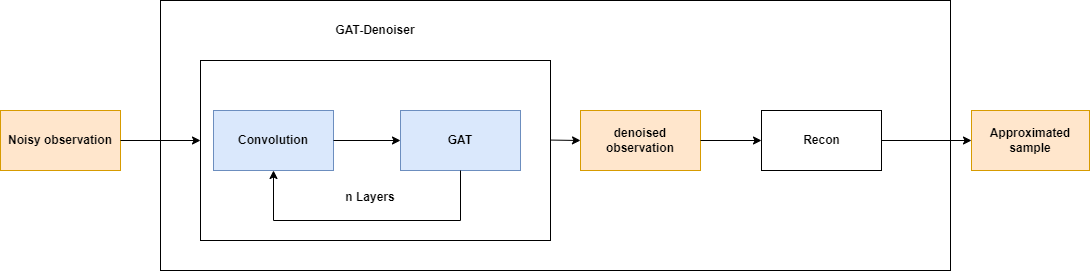
\includegraphics[width=\textwidth]{Overall_GAT-Denoiser_Pipeline.drawio.png}
  \caption{GAT-Denoiser concept}
  \label{fig:overall-concept}
\end{figure}



\paragraph{K-hop neighborhood:}
In GNNs, multiple layers expose the k-hop neighborhood. So for a network with $k$ layers,
network operates on the $k$-hop neighborhood. In GAT-Denoiser, this corresponds
to the layers of GAT. Therefore, if writing from one layer, it is referring to convolution and GAT together.

\section{Layers}

All individual components are introduced and GAT-Denoiser architecture can be defined.
First, the neural network layers will be explained and, second, loss and training.

As defined in Equation~\ref{eq:abstract-model}, $N$ is the number of observation and
$M$ observation dimension. 
Therefore, input (noisy sinogram) will be in $\mathbb{R}^{N \times M}$ as well as output (denoised sinogram). 

In Figure~\ref{fig:architecture-detailed}, detailed GNN architecture can be seen.
It is parametrized with $channels$, $heads$ and $layers$. 
The number of channels in convolution can be increased with parameter $channels$.
Further, $heads$ determine the number of heads used in the GAT layers and parameter 
$layers$ defines how many convolution and GAT layers are stacked together.

\textbf{TODO: In figure everything bold! Replace parameters with c, h and l?}

\begin{figure}[H]
  \centering
  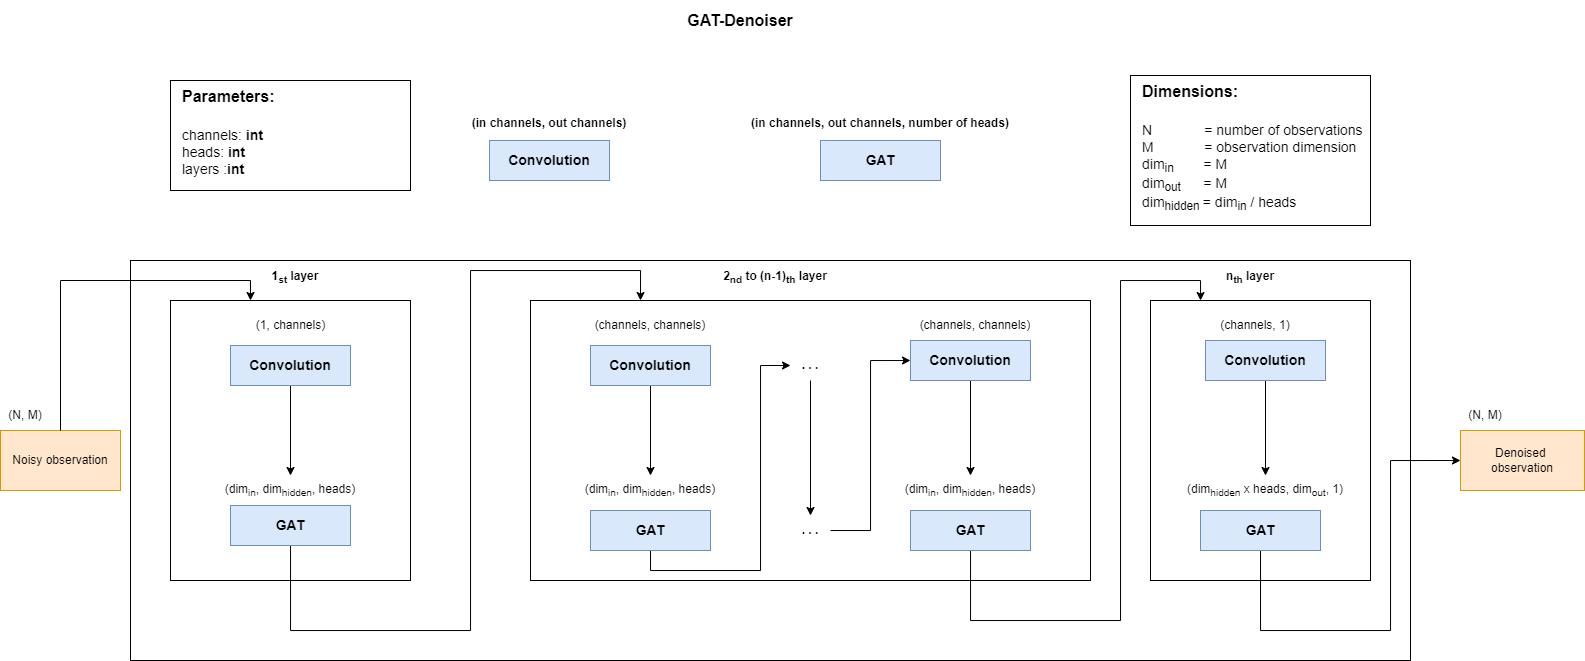
\includegraphics[width=\textwidth]{GAT_Architecture_Detail.drawio.png}
  \caption{Overall GAT-Denoiser architecture}
  \label{fig:architecture-detailed}
\end{figure}


For every layer, first convolution and then GAT is processed. 
Convolution in the whole network was defined with kernel size of 3 and padding 1,
therefore, dimension of convolved signal will not change. 
Convolution can be defined with different parameters, but output signal needs to have 
same dimension as input signal.
Further, additional convolutional channels can be used for learning.
If parameter $channels > 1$, channels are increased in the first convolution layer 
and decreased in the last one.
Parameter $heads$ controls multi-head approach for GAT. Input and hidden dimension
of GAT is $M$ if no heads are used.
If multi-head attention is used, hidden dimension will be set to $M / heads$.
In the last GAT layer, everything gets prepared for output dimension and 
averaging with 1 head is applied.

\section{Training}

\subsection{Loss}

\label{sec:contr_training}
An end-to-end learning approach is used where quality of reconstruction is 
compared in the loss.

Therefore, the outcome of GAT-Denoiser is not directly part of the loss, but first reconstruction will be computed.
Reconstructions can be nicely compared with the $\ell2$-norm:

\begin{equation}
  \label{eq:loss_reco}
  \mathcal{L} = \parallel x_i - \textit{Recon} ( \textit{GAT-Denoiser}(A(x_i, \theta, s) + \eta)) \parallel ^2_2
\end{equation}

As $x_i$ is part of the loss, access to original object is needed during training.

Further, U-Net will be jointly used with FBP as reconstruction. 
Thus, U-Net needs to be first pre-trained with the dataset.
One could also consider training U-Net and GAT-Denoiser jointly.

\textbf{TODO: Add Loss section with part from second loss.}


One could also consider computing loss from GAT-Denoiser output directly, therefore on denoised observation level.
For LoDoPaB-CT dataset, this would mean to compare clean sinogram with denoised sinogram:

\begin{equation}
  \label{eq:loss_sino}
  \mathcal{L}_{sino} = \parallel p_i - \textit{GAT-Denoiser}(A(x_i, \theta, s) + \eta) \parallel ^2_2
\end{equation}
